\documentclass[border=10pt]{standalone}
\usepackage{tikz}
\usetikzlibrary{shapes, arrows.meta, positioning, calc, fit, backgrounds, shadows}

\begin{document}
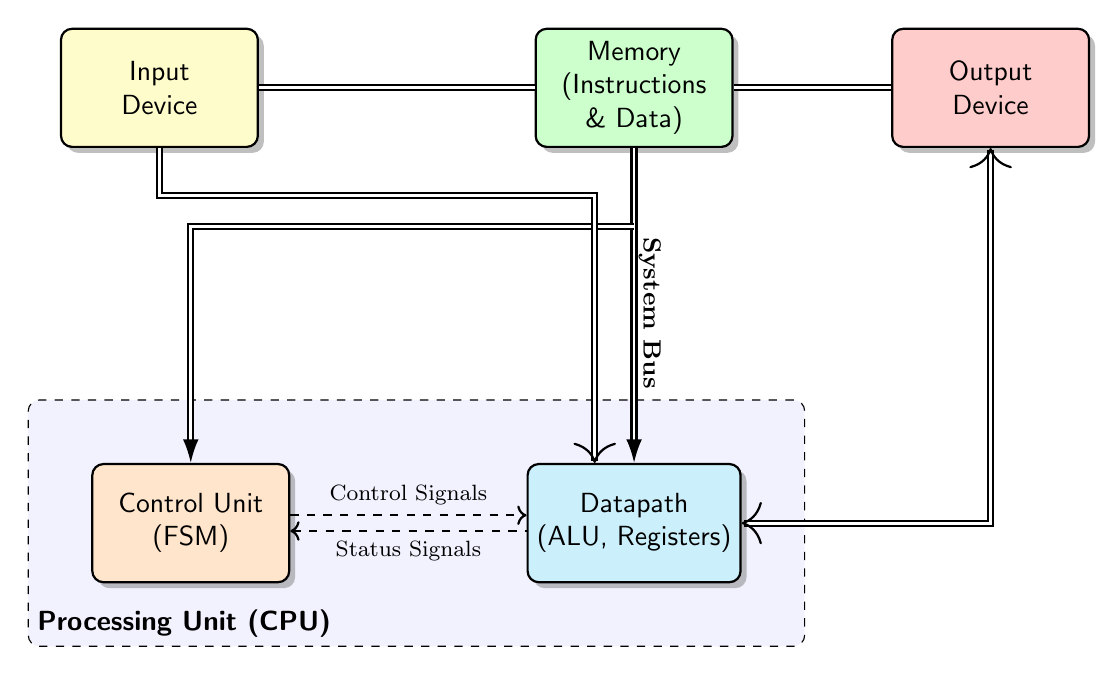
\begin{tikzpicture}[
    font=\sffamily,
    thick,
    box/.style={draw, rounded corners, minimum width=2.5cm, minimum height=1.5cm, align=center, fill=white, drop shadow},
    cpu/.style={draw, rounded corners, inner sep=0.8cm, fill=blue!5, dashed},
    bus/.style={double, double distance=1pt, -{Latex[length=3mm, width=2mm]}},
    bus_line/.style={double, double distance=1pt},
    control_line/.style={dashed, -{Latex[length=2mm, width=1.5mm]}}
]

    % Components
    \node[box, fill=yellow!20] (input) {Input\\Device};
    \node[box, fill=green!20, right=3.5cm of input] (memory) {Memory\\(Instructions \\\& Data)};
    \node[box, fill=red!20, right=2cm of memory] (output) {Output\\Device};

    % CPU Internal Components
    \node[box, fill=cyan!20, below=4cm of memory] (datapath) {Datapath\\(ALU, Registers)};
    \node[box, fill=orange!20, left=3cm of datapath] (control) {Control Unit\\(FSM)};

    % CPU Container
    \begin{scope}[on background layer]
        \node[cpu, fit=(datapath) (control), label={[anchor=south west]south west:\textbf{Processing Unit (CPU)}}] (cpu_box) {};
    \end{scope}

    % Bus Connections
    % Address/Data Bus
    \draw[bus_line] (input.east) -- (memory.west);
    \draw[bus_line] (memory.east) -- (output.west);
    
    % CPU connections to Memory/Bus
    \coordinate (bus_junction) at ($(memory.south) + (0, -1)$);
    \draw[bus_line] (memory.south) -- (bus_junction);
    \draw[bus] (bus_junction) -| (datapath.north);
    \draw[bus] (bus_junction) -| (control.north);
    \draw[bus, <->] (datapath.east) -- ++(1,0) -| (output.south); % Data out
    \path (datapath.north) -- ++(-0.5,0) coordinate (data_bus);
    \draw[bus, <-] (data_bus) -- ++(0,3.4) -| (input.south); % Data in

    % Internal CPU Connections
    \draw[control_line, ->] ($(control.east)+(0,0.1)$) -- node[above, font=\footnotesize] {Control Signals} ($(datapath.west)+(0,0.1)$);
    \draw[control_line, <-] ($(control.east)+(0,-0.1)$) -- node[below, font=\footnotesize] {Status Signals} ($(datapath.west)+(0,-0.1)$);
    
    % Labels
    \node[rotate=270,right=0.2cm of bus_junction, font=\small\bfseries] {System Bus};

\end{tikzpicture}
\end{document}
